\documentclass[14pt,a4paper]{article}
\usepackage{mathtools}
\usepackage{amsmath}
\usepackage{bigints}
\usepackage{mathrsfs}
\usepackage{setspace}
\usepackage{amsfonts}
\usepackage{geometry}
\geometry{a4paper, total = {210mm,297mm},left=35mm, right=25mm,top=25mm,bottom=25mm}
\usepackage{xcolor}
\usepackage{mcode}
\usepackage{listings}
\lstset{basicstyle = \fontsize{11}{12} \selectfont\ttfamily}
\usepackage{subfig}
\usepackage{graphicx}


%Begin document - Vibration Mechanic Systems - Homework 1

\begin{document}
\label{cover}
\begin{center}
	\vspace*{3cm}
	\large{\textbf{ME 5514 VIBRATION MECHANICS SYSTEMS \\ Homework 1}}
	\vfill
	\textbf{Luan Cong Doan} \\ luandoan@vt.edu
	%\vfill
%	Department of Mechanical Engineering \\ Virginia Polytechnic Institute and State University
	\vfill
	\today
\end{center}
%\pagebreak

\label{Answer Sheet}
\label{Vibration Mechanics}
\doublespacing
The system shown is subject to a half-sine pulse input and all initial conditions = 0. Determine the time domain response for 5 seconds $(0 < t < 5)$ using the following methods:\\
\begin{figure}[htp]
	\centering
	\subfloat{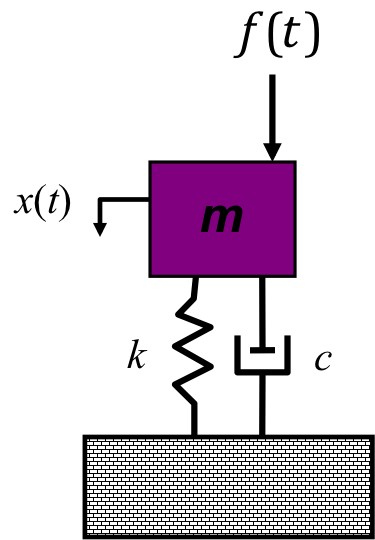
\includegraphics[width=0.45\textwidth]{figure1.jpg}\label{fig:f1}}
	\hfill
	\subfloat{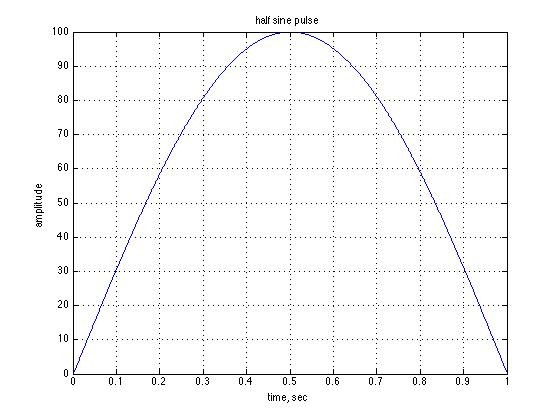
\includegraphics[width=0.45\textwidth]{figure2.jpg}\label{fig:f2}}
\end{figure}\\
with: $m = 100$ lbs; $k = 7$ lb/in; $\zeta = 0.1$\\
\doublespacing
We have the motion differential equation of system:\\
\hspace*{3cm} $m\ddot{x}(t) + c\dot{x}(t) + kx(t) = F_0\sin\omega t$ \\
\hspace*{2.6cm} $ \Leftrightarrow \ddot{x}(t) + 2 \zeta \omega_n \dot{x}(t) + \omega_n^2x(t) = f_0\sin \omega t$\\
with: $\omega_n$ is natural frequency: $\omega_n = \sqrt{\dfrac{k}{m}} = \sqrt{\dfrac{7}{100}} = 0.2646$ rad/s\\
	\hspace*{1cm}	$\zeta$ is damping ratio: $\zeta = \dfrac{c}{2m\omega_n} = 0.1$\\
 \hspace*{1cm} and $f_0 = \dfrac{F_0}{m}$

\begin{enumerate}
	\label{Problem 1}
	\item Compute numerically using the Euler form with time step $\Delta t = 0.1$:\\
	For all initial conditions are 0: $x(0) = x_1(0) = 0; \dot{x}(0) = x_2(0) = 0$.\\
	From half-sine pulse input we could point out that:\\
	\hspace*{1cm} - Amplitude of force is: 100 lbs.\\
	\hspace*{1cm} - Circle time of force is: $T = 2.1 = 2$ seconds\\
	\hspace*{1cm} $\Rightarrow$ force's frequency is: $ f = \dfrac{1}{T} = \dfrac{1}{2} = 0.5$ Hz \\
	\hspace*{0.5cm} Equivalently we have: $\omega = 2\pi f = 2*\pi*0.5 = \pi$ rad/s\\
	\hspace*{0.5cm} We could temporary form the force input model: $f(t) = 100\sin(\omega t + \phi)$\\
	\hspace*{1cm} - For $t_0 = 0, t_1 = 1$ we both have $f(t) = 0 \Rightarrow \phi = 0$\\
	\hspace*{1cm} $\Rightarrow$ The half-sine input equation: $ f(t) = 100\sin(\pi t)$\\
	Applied half-sine pulse input we have the system's motion equation:\\
	\hspace*{2.6cm} $ \ddot{x}(t) + 2 \zeta \omega_n \dot{x}(t) + \omega_n^2x(t) = \sin \pi t$ \hspace{1cm} (because $f_0 = \dfrac{F_0}{m} = \dfrac{100}{100} =1$)\\
	Define $ \begin{cases} x_1 = x(t) \\ x_2 = \dot{x}(t) = \dot{x_1} \end{cases} $ we have: $\begin{cases} \dot{x_1} = x_2 \\ \dot{x_2} = - 2\zeta\omega_nx_2 - \omega_n^2x_1 + \sin\pi t \end{cases} $\\
	
	We have the state-space form of motion equation: \hspace{0.5cm} $\dot{\textbf{x}}(t) = A\textbf{x}(t) + \textbf{f}(t)$\\
	with: $A = \begin{bmatrix} 0&1 \\ -\omega_n^2 & -2\xi\omega_n \end{bmatrix} $; $ \textbf{x} = \begin{bmatrix} x_1 \\ x_2 \end{bmatrix} $; $\textbf{f}(t) = \begin{bmatrix} 0 \\ f_0\cos\omega t \end{bmatrix} $\\
	
	Applying Euler form to motion equation we solution:\\
	\hspace*{3cm}  $x(t_{i+1}) = x(t_i) + Ax(t_i)\Delta t + \textbf{f}(t_i)\Delta t$\\
	Solving problem in \texttt{MATLAB} using the \texttt{ODE45} function we have result:
	\begin{lstlisting}
	TSPAN = 0:0.1:5;
	Y0 = [0;0]; % for initial condition
	[t,y1b] = ode45('num_for_hw1a',TSPAN,Y0);
	figure; plot(t,y1b(:,1));
	xlabel('Time(sec)'); ylabel('Displacement (m)');
	title('Time response for 5 second with f(t) = 100sin\pi t');
	grid on;
	print('vibration_hw1a','-dpng');
	
	function Xdot = num_for_hw1a(t,X)
	m = 100; k = 7; ze = 0.1;
	wn = sqrt(k/m);
	w = pi; F = 100; f = F/m;
	f = [0; f*cos(w*t)];
	A = [0 1; -wn*wn -2*ze*wn];
	Xdot = A*X + f;
	end
	\end{lstlisting}
	
	\label{Figure 1 - Euler form}
	Result is presented in following figure:\\
	\begin{figure}[htp]
		\centering
		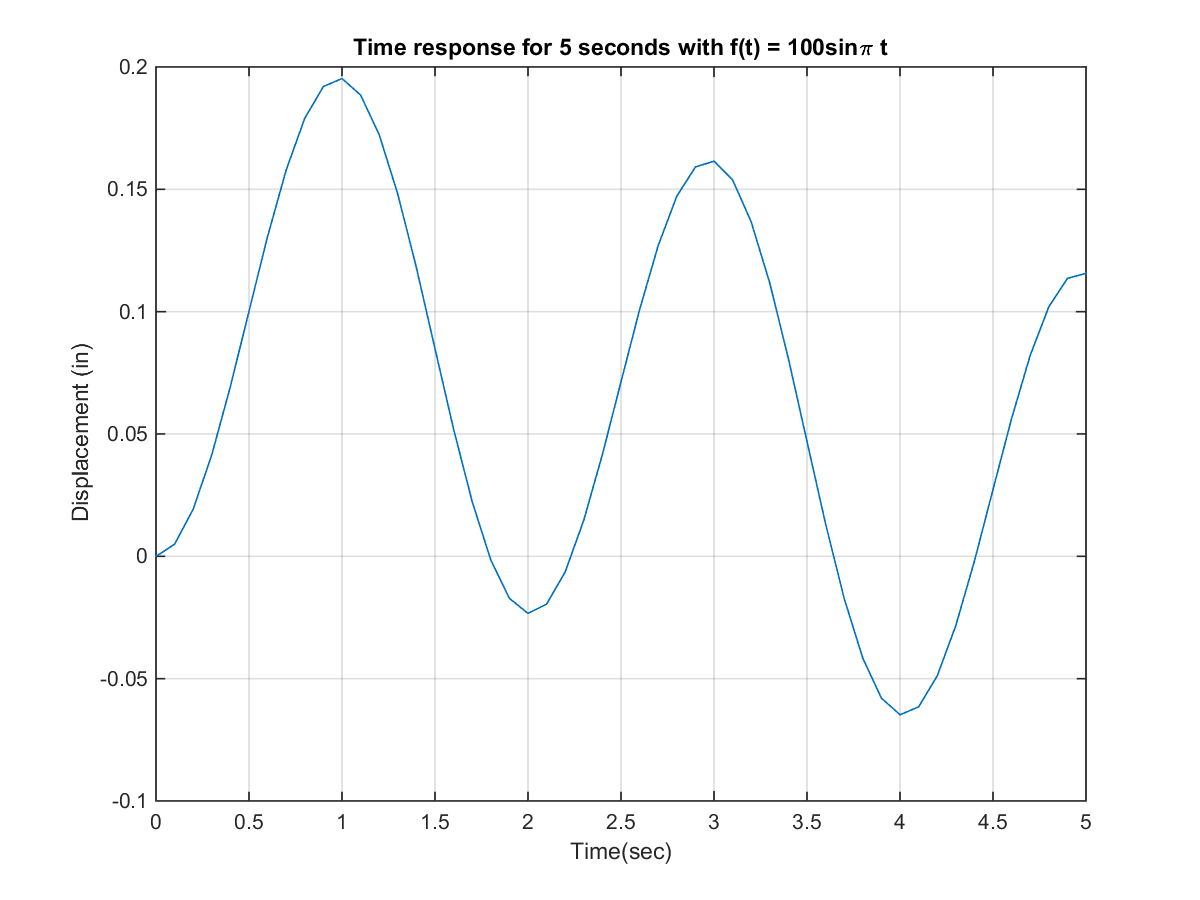
\includegraphics[scale =0.7]{vibration_hw1a.png}
		\caption{Result by applying Euler form for 5 seconds}
	\end{figure}
	\pagebreak
	
	\label{Problem 2 - Harmonic}
	\item Compare with harmonic excitation solution using $f(t) = 100\sin \pi t$ as the input at $t =0$:\\
	System's motion equation: $m\ddot{x}(t) + c\dot{x}(t) + kx(t) = 100\sin\pi t$ \\
	\hspace*{3.7cm} $\Leftrightarrow \ddot{x}(t) + 2 \zeta \omega_n \dot{x}(t) + \omega_n^2x(t) = \sin \pi t$ \hspace{1cm} (*)\\
	we have the particular solution: $x_p(t) = A_s\cos\omega t + B_s\sin\omega t$\\
	with: $A_s = \dfrac{(\omega_n^2 - \omega^2)f_0}{(\omega_n^2 - \omega^2)^2 + (2\zeta\omega_n\omega)^2}$ \hspace{1cm} and \hspace{0.5cm} $B_s = \dfrac{2\zeta\omega_n\omega f_0}{(\omega_n^2 - \omega^2)^2 + (2\zeta\omega_n\omega)^2}$\\
	Overall, we have particular solution:\\
	\hspace*{2cm} $x_p(t) = \dfrac{f_0}{\sqrt{(\omega_n^2 - \omega^2)^2 + (2\zeta\omega_n\omega)^2}} \cos\left( \omega t - \tan^{-1}\dfrac{2\zeta\omega_n\omega}{\omega_n^2 - \omega^2} \right)$
	
	Ignoring the transient response we have solution for (*):\\
	\hspace*{2cm} $x(t) = x_p(t) = \dfrac{f_0}{\sqrt{(\omega_n^2 - \omega^2)^2 + (2\zeta\omega_n\omega)^2}} \cos\left( \omega t - \tan^{-1}\dfrac{2\zeta\omega_n\omega}{\omega_n^2 - \omega^2} \right)$\\
	Solving problem in \texttt{MATLAB} we have solution:
	\begin{lstlisting}
	m = 100; k = 7; ze = 0.1;
	wn = sqrt(k/m);
	w = pi; F = 100; f = F/m;
	X = f/sqrt((wn*wn - w*w)^2 + (2*ze*wn*w)^2);
	phi = atan(2*ze*wn*w/(wn*wn-w*w));
	t = 0:0.1:5;
	xt = X*cos(w*t - phi);
	figure; plot(t,xt); grid on;
	xlabel('Time (sec)'); ylabel('Displacement (in)');
	title('Time response for 5 second with Harmonic motion');
	print('vibration_hw1b','-dpng');
	\end{lstlisting}
	\label{Figure 2 - Harmonic}
	Result is presented in following figure:
	\begin{figure}[htp]
		\centering
		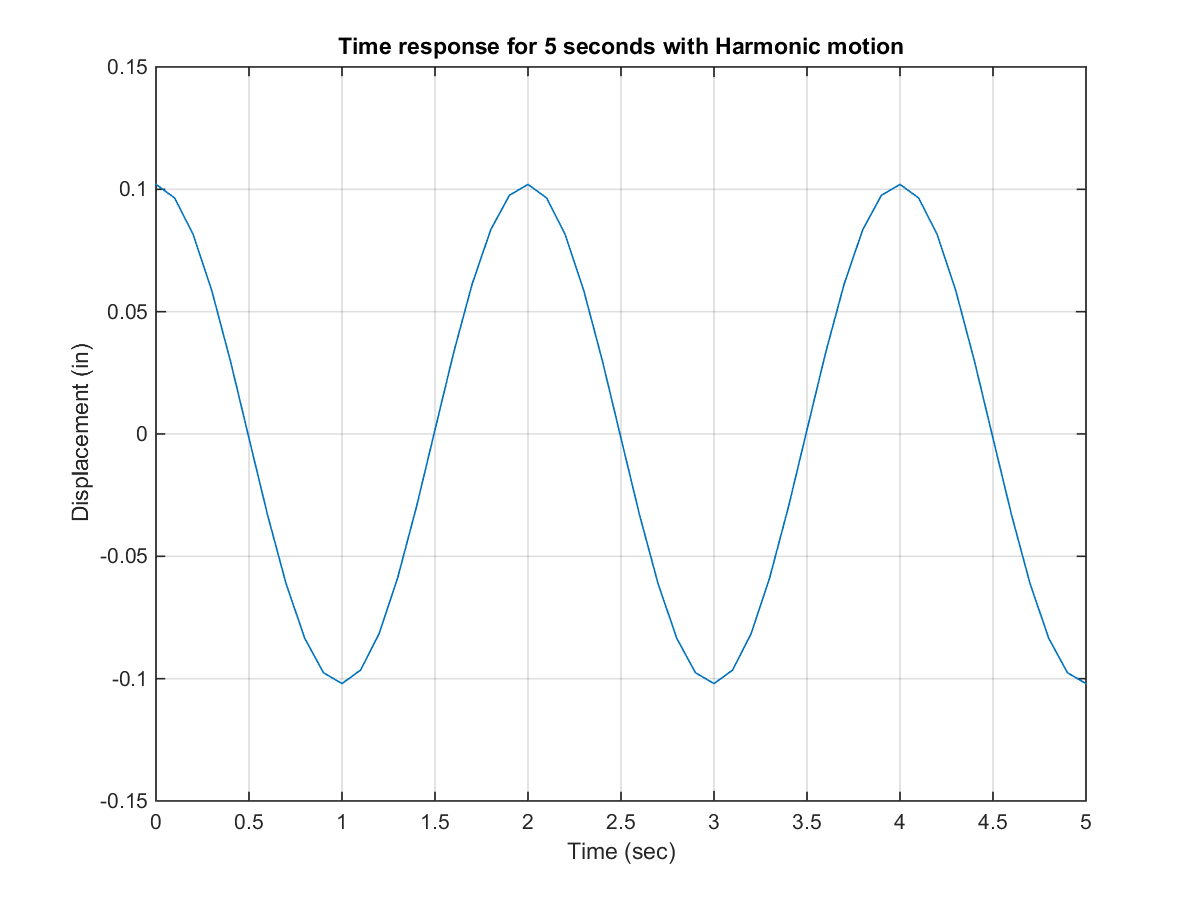
\includegraphics[scale =0.7]{vibration_hw1b.png}
		\caption{Result by applying Harmonic model for 5 seconds}
	\end{figure}
		
	Subtract out a time delayed and negative harmonic input starting at $t = 1$ sec to provide the response beyond 1 sec:
	\begin{lstlisting}
	delta_x = y1a(:,1)' - xt;
	t1 = 0:0.1:1;
	t2 = 0:0.1:4;
	disp1 = zeros(size(t1));
	disp2 = zeros(size(t2));
	for i = 1:size(t1,2)
	    disp1(1,i) =  y1a(i,1);
	end
	for j = 1:size(t2,2)
	    disp2(1,j) = delta_x(1,size(t1,2)+j-1);
	end
	tt = [t1,1+t2];
	disp = [disp1,disp2];
	figure; plot(tt,disp); grid on;
	xlabel('Time (sec)'); ylabel('Displacement (in)');
	title('Time response for 5 seconds');
	print('vibration_hw1b2','-dpng');
	\end{lstlisting}
	\label{Figure 3 - Time response}
	Result is presented in following figure:
	\begin{figure}[htp]
		\centering
		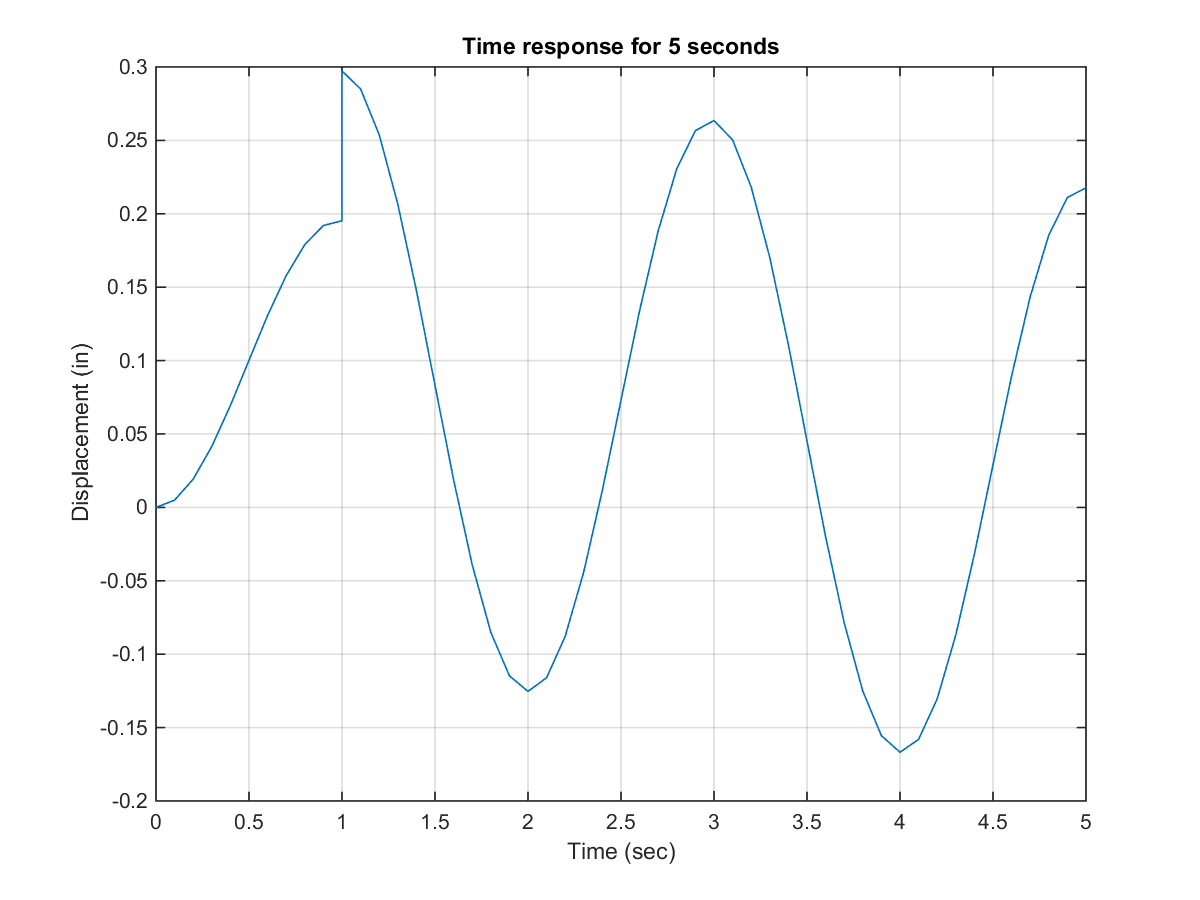
\includegraphics[scale =0.7]{vibration_hw1b2.png}
		\caption{Time response for 5 seconds}
	\end{figure}
		
	\label{Problem 3}	
	\item Compare the maximum amplitude response with the shock response spectrum (\textit{on slide} \#40):\\
%	Using linear super position we have:\\
%	- For $0 \leq t \leq t_1 = 1$ second: $x(t) = \dfrac{F_0}{k} \left(1 - \cos\omega_nt\right)$\\
%	\hspace*{4cm} $\Leftrightarrow \dfrac{x(t)k}{F_0} =  1 - \cos\omega_nt$;\\
%	- For $t > t_1$: $x(t) = \dfrac{F_0}{k} \left[\cos\omega_nt(t-t_1) - \cos\omega_nt\right]$\\
%	\hspace*{1.5cm} $\Leftrightarrow \dfrac{x(t)k}{F_0} =  \cos\omega_nt(t-t_1) - \cos\omega_nt$;\\
%	Solving for $\dfrac{x(t)k}{F_0}$ in \texttt{MATLAB} we have:
%	\begin{lstlisting}
%xtkFo = zeros(1,size(t1,2)+size(t2,2)-1);
%for i = 1:size(t1,2)
%xtkFo(1,i) =  1 - cos(wn*t1(i));
%end
%for j = 1:size(t2,2)
%xtkFo(1,size(t1,2)-1+j) = cos(wn*t2(i))*(t2(i)-1) + cos(wn*t2(i));
%end
%figure; plot(t,xtkFo); grid on;
%xlabel('t1/T'); ylabel('(x(t)k/Fo)_max');
%title('Shock Response Spectra');
%print('vibration_hw1c','-dpng');
%	\end{lstlisting}
%	Result is presented in following figure:
%	\begin{figure}[htp]
%		\centering
%		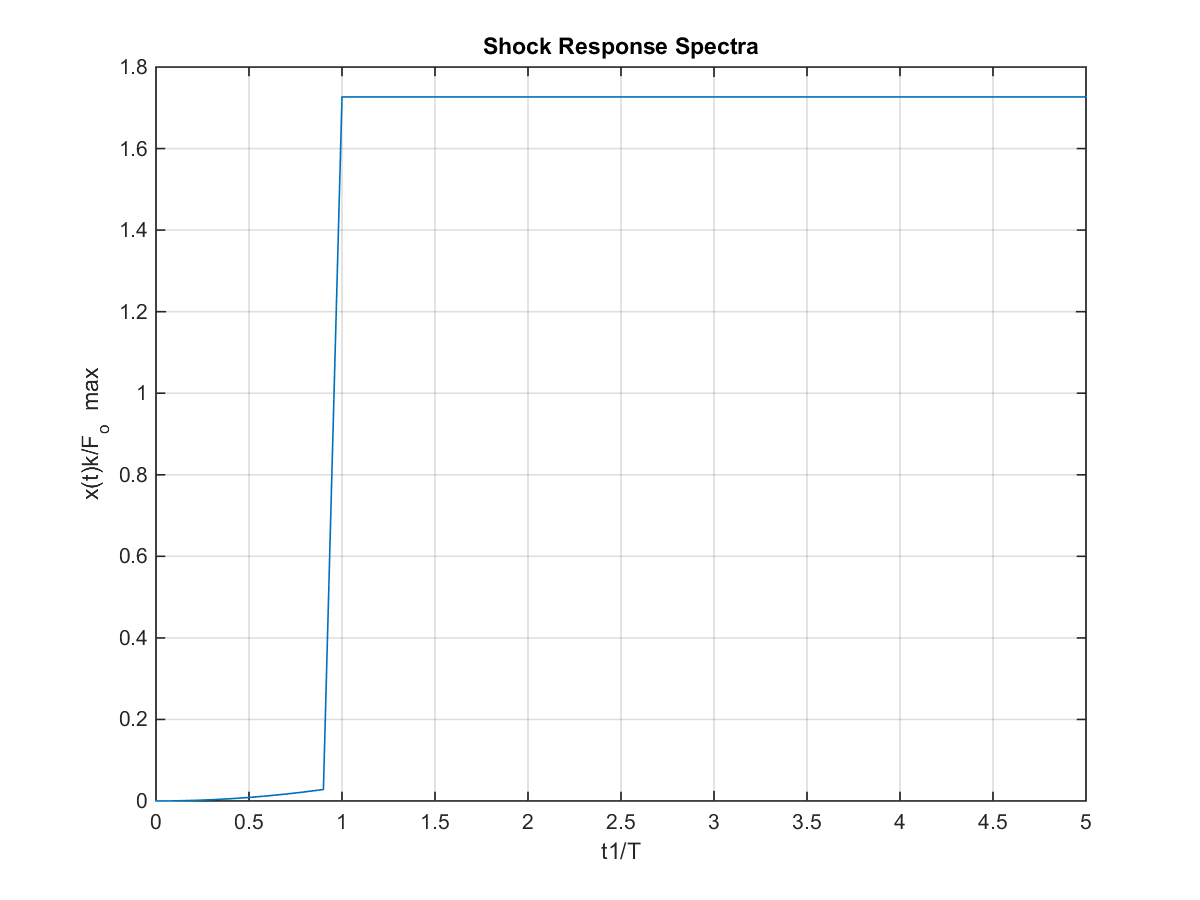
\includegraphics[scale =0.7]{vibration_hw1c.png}
%		\caption{Shock Response Spectra}
%	\end{figure}
	System is undamped ($\zeta = 0.1 < 1$) so based on slide \#40 we have the maximum magnitude response in 5 second is the highest peak on plot of figure 3.\\ 
	Based on \texttt{MATLAB} result, we have \textbf{\textit{maximum magnitude response}} is \textbf{\texttt{0.2973}} at time step \textbf{\textit{t = 1}} second.\\
\end{enumerate}

\end{document}